\clearpage

\section{Class 使用方法}


\par 紙張的選擇:「B5」或者「b5paper」他們彼此是完全相同的。
\par 注意:此「b5paper」為 JIS B5 規格(寬 182mm,高 257mm)。
\par 還可以選擇「test」選項調用卷子畫幅,注意,使用「test」時需使用 \verb+\pagestyle{empty} + 消除書眉和頁碼,
以方便pdfcrop工具進行剪裁。
\par 不推薦使用 「twocolumn」選項,因其容易引起版面混亂。現推薦使用 「multirow」和「multicol」,通過
調用{\verb+\begin{multicols}{2} xxxx \end{multicols} + } 環境,來使用雙欄。

\par 本模板和 「geometry」宏包不兼容,强行使用會出現版面混亂。在 settings.sty 中調整版面,手動設置
文本行長(textwidth)。

\par 應使用 \verb+\setlength{\xxx}{5 mm} + 的方式設置長度變量,如采用\verb+\setlength\xxx{5mm} + 的
方式可能不會成功。例如設置段落縮進,應采用:{\verb+ \setlength{\parindent}{2 zw} + }
而不推薦大家使用:\\
{\uwave{\color{red}\verb+ \setlength\parindent{2 zw} + }}


%\clearpage

\section{為up{\LaTeX}配置本地字體}

\subsection{字體實現的三種思路。}
\par\noindent
思路一:通過NFSS設置方法,將已有的tfm及同名vf映射到本地字體。\\
優點:簡單方便,不產生新的vf和tfm,僅適用於臨時占用。\\
缺點:會占用系統預設的tfm和vf。\\[5mm]
思路二:使用PXcopyfont工具包為本地字體複製配套的tfm和vf。\\
優點:為每一個本地字體都配置單獨的vf及tfm,可以避免同系統自帶的tfm及vf撞車;\\
\hspace{3zw}便於移植到下一台計算機。\\
缺點:占用硬盤資源大。配置難度大。\\[5mm]
思路三:使用Jfmutil工具包為本地字體創建全新的tfm和vf。\\
優點:可以自定義禁則。便於移植到下一台計算機。\\
缺點:配置難度太大,禁則編寫難度太高,往往不容易成功。


\subsection{簡體中文字體宏包}
\par
使用\verb+ctex+宏包可以調用Windows/OS X/Linux 本地字体。
使用此package前請先閲讀ctex.pdf 手冊,目前中文繁體支持仍然很差,
除楷體和宋體外,隸書僅支持簡體中文使用。
\begin{lstlisting}[firstnumber=1]
\usepackage[fontset=windows]{ctex}
%\usepackage[fontset=adobe]{ctex}
\end{lstlisting}


\subsection{{up\LaTeXe}字體設置方法(NFSS)}

\par{}使用 八登崇之 PXcopyfont 工具包。(見附件 PXcopyfont 文件夾。)
\par{}安裝 perl 工具包。Windows 10 系統可以下載使用 {ActivePerl}。

\subsubsection*{案例一創建 {kleePro} 虛擬字體和TFM文件}

(請勿照抄此案例。)

\par{}{\bfseries{Windows系統}}在記事本中寫入以下語句,另存為 \uwave{\red{MK KLEE.BAT}}。
\begin{lstlisting}[firstnumber=1]
perl pxcopyfont.pl -o upjisr-h klee-m-jy2 r-klee-m-jy2 r-klee-m-jy2x
perl pxcopyfont.pl -o upjisr-v klee-m-jt2 r-klee-m-jt2
perl pxcopyfont.pl -o jis klee-m-jy1 r-klee-m-jy1
perl pxcopyfont.pl -o jis-v klee-m-jt1 r-klee-m-jt1
perl pxcopyfont.pl -o upjisr-h klee-db-jy2 r-klee-db-jy2 r-klee-db-jy2x
perl pxcopyfont.pl -o upjisr-v klee-db-jt2 r-klee-db-jt2
perl pxcopyfont.pl -o jis klee-db-jy1 r-klee-db-jy1
perl pxcopyfont.pl -o jis-v klee-db-jt1 r-klee-db-jt1
\end{lstlisting}

\par{}保存後,直接雙擊執行。不能用管理員權限,否則進入system32系統文件夾下了。
\par{}現在打開
{\color{red}C:$\backslash$texlive$\backslash$texmf-local$\backslash$fonts$\backslash$vf},
新建klee文件夾,將vf字體複製進去。
\par{}打開
{\color{red}C:$\backslash$texlive$\backslash$texmf-local$\backslash$fonts$\backslash$tfm},
新建klee文件夾,將tfm文件複製進去。
\par{}執行\red{mktexlsr}刷新{\TeX}文件樹。


\subsubsection*{案例二創建 {kleePro} 配置文件}

(請勿照抄此案例。)

\par{}參考{doratex}的博客,在{mysample.tex}中寫入以下語句,使用
{\color{red}\verb+{ptex2pdf -l -u  mysample}+}
進行編譯:
\begin{lstlisting}[firstnumber=1]
%#!使用uplatex 編譯
\documentclass[uplatex]{jsarticle}
\usepackage{plext}% 縦組用
\pagestyle{empty}
%%% klee ファミリーに m と db のシリーズを定義
\DeclareFontFamily{JY2}{klee}{}
\DeclareFontFamily{JT2}{klee}{}

\DeclareFontShape{JY2}{klee}{m}{n}{<->s*[0.924690]klee-m-jy2}{}
\DeclareFontShape{JY2}{klee}{m}{it}{<->ssub*klee/m/n}{}
\DeclareFontShape{JY2}{klee}{m}{sl}{<->ssub*klee/m/n}{}
\DeclareFontShape{JY2}{klee}{m}{sc}{<->ssub*klee/m/n}{}
\DeclareFontShape{JT2}{klee}{m}{n}{<->s*[0.924690]klee-m-jt2}{}
\DeclareFontShape{JT2}{klee}{m}{it}{<->ssub*klee/m/n}{}
\DeclareFontShape{JT2}{klee}{m}{sl}{<->ssub*klee/m/n}{}
\DeclareFontShape{JT2}{klee}{m}{sc}{<->ssub*klee/m/n}{}

\DeclareFontShape{JY2}{klee}{db}{n}{<->s*[0.924690]klee-db-jy2}{}
\DeclareFontShape{JY2}{klee}{db}{it}{<->ssub*klee/db/n}{}
\DeclareFontShape{JY2}{klee}{db}{sl}{<->ssub*klee/db/n}{}
\DeclareFontShape{JY2}{klee}{db}{sc}{<->ssub*klee/db/n}{}
\DeclareFontShape{JT2}{klee}{db}{n}{<->s*[0.924690]klee-db-jt2}{}
\DeclareFontShape{JT2}{klee}{db}{it}{<->ssub*klee/db/n}{}
\DeclareFontShape{JT2}{klee}{db}{sl}{<->ssub*klee/db/n}{}
\DeclareFontShape{JT2}{klee}{db}{sc}{<->ssub*klee/db/n}{}

\DeclareRobustCommand\kleem{\kanjifamily{klee}\kanjiseries{m}\selectfont}
\DeclareRobustCommand\kleedb{\kanjifamily{klee}\kanjiseries{db}\selectfont}

% dvipdfmx special の発行
\AtBeginDvi{%
  \special{pdf:mapline klee-m-jy2    UniJIS2004-UTF16-H FOT-KleePro-M.otf}%
  \special{pdf:mapline klee-m-jt2    UniJIS2004-UTF16-V FOT-KleePro-M.otf}%
  \special{pdf:mapline klee-db-jy2   UniJIS2004-UTF16-H FOT-KleePro-DB.otf}%
  \special{pdf:mapline klee-db-jt2   UniJIS2004-UTF16-V FOT-KleePro-DB.otf}%
}

\begin{document}
\parbox<y>{22zw}{%
{\kleem{}(*クレーミディアムの横組サンプル、「約物の“テスト”」。*)}\par
{\kleedb{}(*クレーデミボールドの横組サンプル、「約物の“テスト”」。*)}}
\vspace{5mm}
\parbox<t>{12zw}{%
{\kleem{}(*クレーミディアムの縦組サンプル、「約物の〝テスト?」。*)}\par
{\kleedb{}(*クレーデミボールドの縦組サンプル、「約物の〝テスト?」。*)}}
\end{document}
\end{lstlisting}

\begin{figure}[H]
\par\quad\marg{出力例:}
\begin{center}
\fbox{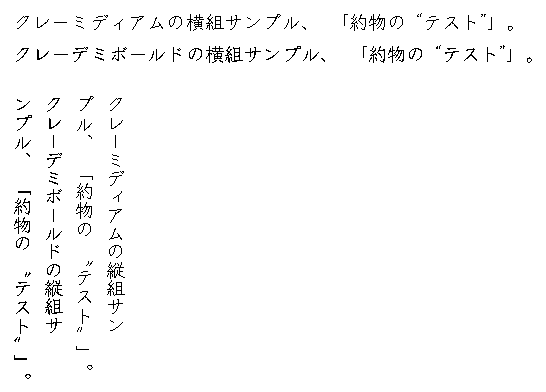
\includegraphics[width=0.6\textwidth]{figures/06.pdf}}
\end{center}
\end{figure}

%\clearpage
\subsection{簡體中文本地字體}

\par{}參照前文
配置虛擬字體和tfm。然後指定mapline為{UniGB-UTF16-H}和{UniGB-UTF16-V},
或者{UniGB-UCS2-H}和{UniGB-UCS2-V}。 或者使用 {unicode}作爲{mapline}。
示例如下:

\begin{lstlisting}[firstnumber=1]
  \special{pdf:mapline fzks-m-jy2   unicode  FZKSGBXS10.ttf}% 方正楷書 (*GB18030-S10*)版
  \special{pdf:mapline fzks-m-jt2   unicode  FZKSGBXS10.ttf -w 1}% -w 1 表示垂直排版模式
  \special{pdf:mapline fzks-sip-m-jy2   unicode  FZKaiS(SIP).TTF}%方正楷書(*S-SIP(CJK-B版)*)
  \special{pdf:mapline fzks-sip-m-jt2   unicode  FZKaiS(SIP).TTF -w 1}%
  \special{pdf:mapline fzxss-m-jy2   UniGB-UTF16-H  FZXSSGBX.TTF}% 方正新書宋 GB18030
  \special{pdf:mapline fzxss-m-jt2   UniGB-UTF16-V  FZXSSGBX.TTF}%
\end{lstlisting}

\subsection{使用{Pxchfon}宏包配置日文版思源字體}
\par{}在{mysample.tex}中寫入以下語句:

\begin{lstlisting}[firstnumber=1]
\usepackage[uplatex,deluxe]{otf}               % 多字重支持
%\usepackage[sourcehan]{pxchfon}                 % 不使用 JIS2004 字形
\usepackage[sourcehan,prefer2004jis]{pxchfon}    %   使用 JIS2004 字形

\setminchofont{SourceHanSerif-Medium.otf}
\setlightminchofont{SourceHanSerif-Regular.otf}
\setboldminchofont{SourceHanSerif-Bold.otf}
\setgothicfont{SourceHanSans-Medium.otf}
\setmediumgothicfont{SourceHanSans-Regular.otf}
\setboldgothicfont{SourceHanSans-Bold.otf}
\setxboldgothicfont{SourceHanSans-Heavy.otf}
\setmarugothicfont{SourceHanSans-Regular.otf}
\end{lstlisting}

(行5 - 12 是 sourcehan 選項時預設的,與之等價,詳見 pxchfon.pdf)

\begin{table}[H]
\begin{center}
\caption{pxchfon 宏包等價命令}
{\fontsize{8pt}{12}\selectfont\ttfamily
\begin{tabular}{|l|l|l|}
 \hline
 \multicolumn{1}{|c|}{OTF/TTF 命令} & \multicolumn{1}{|c|}{TTC 命令} & \multicolumn{1}{|c|}{用途} \\ \hline
$\backslash$setminchofont\{*.otf/*.ttf\} & $\backslash$setminchofont[番號]\{*.ttc\} & 設置正文明朝體;\\
$\backslash$setlightminchofont\{*.otf/*.ttf\} & $\backslash$setlightminchofont[番號]\{*.ttc\} & 設置細明朝體;\\
$\backslash$setboldminchofont\{*.otf/*.ttf\} & $\backslash$setboldminchofont[番號]\{*.ttc\} & 設置粗明朝體;\\
$\backslash$setgothicfont\{*.otf/*.ttf\} & $\backslash$setgothicfont[番號]\{*.ttc\} & 設置哥特體(細黑體);\\
$\backslash$setmediumgothicfont\{*.otf/*.ttf\} & $\backslash$setmediumgothicfont[番號]\{*.ttc\} & 設置中等哥特體;\\
$\backslash$setboldgothicfont\{*.otf/*.ttf\} & $\backslash$setboldgothicfont[番號]\{*.ttc\} & 設置粗哥特體;\\
$\backslash$setxboldgothicfont\{*.otf/*.ttf\} & $\backslash$setxboldgothicfont[番號]\{*.ttc\} & 設置特粗哥特體;\\
$\backslash$setmarugothicfont\{*.otf/*.ttf\} & $\backslash$setmarugothicfont[番號]\{*.ttc\} & 設置丸書體(即圓體)。\\ \hline
\end{tabular} }
\end{center}
\end{table}


\subsection{東亞字體CMAP簡介}
\par{}CMAP是對字符映射起到索引作用的文件。(見表3)

\subsection{CID-Key和CID符號}

\par{}{up\LaTeXe}自帶一些系統命令,可以調用系統字體(如小塚明朝 kozuka-pr6n)的CID字和符號。
具體CID編號需檢索技術文檔{5078.Adobe-Japan1-6.pdf},網頁搜索即可獲取。相關示例(見表4)


\begin{table}[H]
\caption{東亞字體CMAP簡介}
{\fontsize{8pt}{12}\selectfont\ttfamily
\begin{tabular}{|c|l|l|c|l|}
\hline
 \multicolumn{1}{|c|}{言 語} & \multicolumn{1}{|c|}{CMAP(橫)}%
  &\multicolumn{1}{|c|}{CMAP(縱)}& \multicolumn{1}{|c|}{工具引擎} & \multicolumn{1}{|c|}{備注} \\ \hline
日本語& 2004-H & 2004-V & {p\LaTeX}、{p\TeX} & 適用於JIS2004字形 \\
日本語& UniJIS-UTF16-H & UniJIS-UTF16-V & {up\LaTeX}、{Up\TeX} & 適用於JIS90字形 \\
日本語& UniJIS2004-UTF16-H & UniJIS2004-UTF16-V & 同上 & 適用於JIS2004字形 \\
日本語& UniSourceHanSansJP-UTF16-H & UniSourceHanSansJP-UTF16-V & 同上 & 源ノ角ゴシック (思源黑體日版) \\
日本語& UniSourceHanSerifJP-UTF16-H & UniSourceHanSerifJP-UTF16-V & 同上 & 源ノ明朝(思源明體日版) \\ \hline
簡體中文& UniSourceHanSansCN-UTF16-H & UniSourceHanSansCN-UTF16-V & 同上 & 思源黑體 \\
簡體中文& UniSourceHanSerifCN-UTF16-H & (無,用unicode替代) & 同上 & 思源宋體 \\
簡體中文& UniGB-UTF16-H & UniGB-UTF16-V & 同上 & 適用於簡體 \\
簡體中文& UniGB-UCS2-H & UniGB-UCS2-V & 同上 &  \\ \hline
繁體中文& UniSourceHanSansTW-UTF16-H & (無,用unicode替代) & 同上 & 思源黑體台版 \\
繁體中文& UniSourceHanSerifTW-UTF16-H & (無,用unicode替代) & 同上 & 思源宋體台版 \\
繁體中文& UniCNS-UTF16-H & UniCNS-UTF16-V & 同上 & 適用於繁體 \\
繁體中文& UniCNS-UCS2-H & UniCNS-UCS2-V & 同上 &  \\ \hline
韓國語& (無,用unicode替代) & (無,用unicode替代) & 同上 & 思源黑體韓版 \\
韓國語& 同上 & 同上 & 同上 & 思源明體韓版 \\
韓國語& UniKS-UTF16-H & UniKS-UTF16-V & 同上 &  \\ \hline
\end{tabular} }
\end{table}



\begin{table}[H]
\begin{center}
\caption{Adobe-Japan1-6 使用CID鍵調用特殊符號 示例}
\begin{tabular}{|c|c|c|}
\hline
 入例 & 出例 & 說明\\ \hline
\verb+\CID{1260}+ & \CID{1260} & “永”字 \\
\verb+\CID{119}+ & \hskip.3zw\CID{119} & 垂直磅點,用於縱書 \\
\verb+\CID{8015}+ & \CID{8015} & 圓角方框 \\
\verb+\CID{779}+ & \CID{779} & 圓圈號 \\
\verb+\CID{731}+ & \CID{731} & 上三角 \\
\verb+\CID{733}+ & \CID{733} & 下三角 \\ \hline
\end{tabular}
\end{center}
\end{table}


\clearpage
\section{欄目的整形}


\begin{center}
{\fontsize{8pt}{12}\selectfont\ttfamily
正文字號 16 pt 時,各欄間距對版心的約束\\[2mm]
\begin{tabular}{|c|c|c|c|c|}
\hline
序號	&	欄目个数	&	正文行距	&	版心寬度約束	&	内邉框寬度  \\ \hline
1	&	14	&	25	&	341	&	350	\\
2	&	14	&	26	&	354	&	364	\\
3	&	14	&	27	&	367	&	378	\\
4	&	14	&	28	&	380	&	392	\\
5	&	14	&	29	&	393	&	406	\\
6	&	14	&	30	&	406	&	420	\\ \hline
7	&	15	&	25	&	366	&	375	\\
8	&	15	&	26	&	380	&	390	\\
9	&	15	&	27	&	394	&	405	\\
10	&	15	&	28	&	408	&	420	\\
11	&	15	&	29	&	422	&	435	\\
12	&	15	&	30	&	436	&	450	\\ \hline
13	&	16	&	25	&	391	&	400	\\
14	&	16	&	26	&	406	&	416	\\
15	&	16	&	27	&	421	&	432	\\
16	&	16	&	28	&	436	&	448	\\
17	&	16	&	29	&	451	&	464	\\
18	&	16	&	30	&	466	&	480	\\
 \hline
\end{tabular}\\[2mm]
}
\end{center}

此表格在換算欄目関係時非常有用。

同欄目数,相鄰行距可以公用一個内邉框寬度。
如:14欄29pt和14欄30pt,可公用406pt作爲内邉框寬度。

相鄰欄目,相差2pt的可以公用一個内邉框寬度,
如:14欄30pt和15欄28pt,可公用420pt作爲内邉框寬度。

當然啦,在實際設置中,内邉框寬度應比欄目寬度總和略大1至2pt。
在大行距時,這種差異不明顯。在小行距時,需要特別調整,使其基本吻合。

%\endinput

\clearpage

\begin{center}

\begin{minipage}<y>[htpb]{144mm}
%\vspace*{-20mm}

\begin{tikzpicture}%[overlay]
	\foreach \i in {540,510,...,150}{% 起始点 + 52pt 每栏 从右往左
	%	起始點 416+25.5pt
		\draw [ color=red ] (\i pt, 15)--(\i pt, 22);
	}% 絲欄 

\node [below,rectangle]  at%
		(525pt,22) {\hbox{\tate\gt\ebseries\large{例一}}};

	
\node [below,rectangle]  at%
		(529pt,21) {\hbox{\tate\LARGE\gtfamily{滿帋荒唐言}\quad{一把辛酸淚}}};

\node [below,rectangle]  at%
		(499pt,21) {\hbox{\tate\LARGE\gtfamily{都云作者痴}\quad{誰解其中味}}};
\node [below,rectangle]  at%
		(510pt,17.5) {\hbox{\tate\mgfamily\small\red{此是第一首標題詩。}}};

\node [below,rectangle]  at%
		(435pt,22) {\hbox{\tate\gt\ebseries\large{例二}}};

\node [below,rectangle]  at%
		(430pt,21) {\hbox{\tate\LARGE\gtfamily{滿帋荒唐言}\quad{一把辛酸淚}}};

\node [below,rectangle]  at%
		(400pt,21) {\hbox{\tate\LARGE\gtfamily{都云作者痴}\quad{誰解其中味}}};
\node [below,rectangle]  at%
		(411pt,17.5) {\hbox{\tate\mgfamily\small\red{此是第一首標題詩。}}};

\node [below,rectangle]  at%
		(345pt,22) {\hbox{\tate\gt\ebseries\large{例三}}};

\node [below,rectangle]  at%
		(345pt,21) {\hbox{\tate\LARGE\gtfamily{滿帋荒唐言}\quad{一把辛酸淚}}};

\node [below,rectangle]  at%
		(315pt,21) {\hbox{\tate\LARGE\gtfamily{都云作者痴}\quad{誰解其中味}}};
\node [below,rectangle]  at%
		(326pt,17.5) {\hbox{\tate\mgfamily\small\red{此是第一首標題詩。}}};

\end{tikzpicture}%

{\huge\gt{行間注精調}}
\large

\vskip\baselineskip

行間注使用 pxrubrica 宏包調用,相関内容上網搜索或者察看 pxrubrica.pdf 手冊。

{\bf{例一}}:文本左移不彀,導致侵右側限。

解決辦法:1、使用命令平移頁面。2、修改糸欄的起點和步進,使糸欄去將就文本。

3、在段落之前使用\verb+\vskip3pt+或者\verb+\vspace*{3pt}+,数値視實際而定。

{\bf{例二}}:文本右移不彀,導致侵左側限。

解決辦法:1、2、同上。3、在段落之前使用\verb+\vskip-3pt+ 或者 \verb+\vspace*{-3pt}+,数値視實際而定。

{\bf{例三}}:正常的文本應該是這樣。漢字中心位於欄目中心,左右兩側空白相等。
行間注文寬度8pt,正文漢字寬度15pt(因 Cjascale 參数引起的本文縮小),這樣當行距=欄距=30pt 時,
文本剛好位於欄目中心,且行間注不侵限。


\end{minipage}
\end{center}

\clearpage

